\scanpage{172}

donne

\deleted{\(\unsure{g_n\geq 3}\)}
\[
\underbrace{\underbrace{(2-2g_n)}_{\text{EP de }\widehat U_n}-3n}_{\text{EP}_{!}\text{ de }U_n}
=n^2\left(\underbrace{\underbrace{2}_{\text{EP de }\unsure{\widehat U_1}}-3}_{\text{EP de }U_1}\right)
\]

i.e.
\[
\inserted{2(g_n-1)=n^2-3n}
\qquad
\deleted{\unsure{2-2g_n=-n^2}}
\qquad \text{i.e.}
\]
\[
\text{(369)}\qquad g_n=\deleted{\unsure{2+}}1+\frac12 n(n-3)
\]

Donc on a
\[
\text{(370)}\qquad g_1=g_2=0,\quad g_3=1,\quad g_n>1\quad\text{si }n\geq\deleted{\unsure{3}}\inserted{4}.
\]

En tout état de cause, tous les $U_n$ sont anabéliens, et $\overline{\mathrm m}$ les $\widehat U_n$ pour $n\geq4$.

Si le yoga \inserted{``\uline{anabélien}''} développé dans la première partie de ces notes est valable, les \deleted{\unsure{existence}} \deleted{(ou la non existence) de} points rat/$\mathbb Q$ d'une courbe $U_n$ \deleted{\unsure{s'expliquent par|s'expriment par}} \inserted{correspondent} aux \uline{scindages} de l'extension de groupes profinis

\begin{samepage}
\noindent (371)
\diagram{\begin{tikzcd}[column sep=small]
1 \arrow[r] & \Pi_1(U_{n\overline{\mathbb Q}}) \arrow[r] &
\underset{\inserted{\substack{\unsure{\cap}\\\Pi_1(\unsure{U_1})\simeq\unsure{M_{0,3}^{!}}}}}{\Pi_1(U_n)} \arrow[r] & \Gamma_{\mathbb Q} \arrow[r] & 1
\end{tikzcd}}
\end{samepage}

qui soient distincts des ``scindages à l'infini'' (localisés en les \inserted{3n} pts à l'infini de $U_n$\ldots), ou encore, les scindages tels que \inserted{le \uline{centralisateur} de} $(\Gamma_{\mathbb Q}^{+}=\operatorname{Ker}(\Gamma_{\mathbb Q}\xrightarrow{\chi}\widehat{\mathbb Z}^{*}))$ dans $\Pi_1(U_n)$ soit réduit à $\{1\}$. Donc -- si le ``th.

\scanpage{173}
\mspage{734}

de Fermat'' est bel et bien valable (pour $U_n$, disons), il devrait se \unsure{refléter|réfléter} par la non-existence d'un tel scindage. D'ailleurs, si nous \unsure{arrivions} à prouver l'inexistence de scindages de (371) autres que ceux ``provenant des pts à l'infini'', le th. de Fermat serait prouvé pour $U_n$, même sans avoir établi le ``yoga anabélien'' (dont une démonstration semble bien hors d'atteinte!). Or il n'est nullement exclu qu'une analyse assez poussée de $M_{0,3}$ et $N_{1,1}$ dans la direction actuelle -- impliquant aussi des ``approximations'' de plus en plus fines de $\Pi_1(U_n)$ et de la structure d'extension (371), permette finalement de prouver l'inexistence de scindages ``non triviaux'' de (371), pour tout $n\geq3$. Chaque nouvel affinement des ``approximations de Lie'' de $M_{0,3}$ devrait amener un réexamen de la situation (371) et de la question de ses scindages, dans l'optique d'une démonstration éventuelle des ``th. de Fermat''.

\scanpage{174}

Il s'impose de partir d'approximations de Lie au moins aussi fines que \unsure{celles|celle} du présent \S, qui apparaît comme l'approximation ``minima'' dans laquelle on puisse exprimer ``algébriquement'' la tour des courbes de Fermat, \deleted{\unsure{où}} comme on l'a vu dans 13\textsuperscript{o}), à partir de $M_{0,3}\subset M_{0,3}^{\text{ét}}$.

Tenant compte des opérations de $\mathfrak S_3$ sur $U_n$, la suite exacte (371) se plonge d'ailleurs dans une suite exacte plus riche

\begin{samepage}
\noindent (372)
\diagram{\begin{tikzcd}[column sep=small]
1 \arrow[r] & \Pi_1(U_{n\overline{\mathbb Q}}) \arrow[r] &
\underset{\inserted{\substack{\cap\\\Pi_1(U_1,\mathfrak S_3)\simeq M_{0,3}}}}{\Pi_1(U_n,\mathfrak S_3)} \arrow[r] & \Gamma_{\mathbb Q}\times\mathfrak S_3 \arrow[r] & 1,
\end{tikzcd}}
\end{samepage}

et les calculs faits dans le présent \S\ semblent suggérer que cette structure d'extension plus riche jouera un rôle important.

Du point de vue de l'approximation de Lie de $M_{0,3}$ développée dans le présent \S, il y a lieu de remplacer la structure d'extension (\unsure{372}) par une structure quotient moins fine, en divisant par un sous-groupe invariant de $\Pi_1(U_n,\mathfrak S_3)$ contenu dans

\scanpage{175}
\mspage{735}

$\Pi_1(U_n,\overline{\mathbb Q})$, savoir l'intersection dans $M_{0,3}$ de ce groupe avec $[\widehat\Pi_{0,3},\widehat\Pi_{0,3}]$. On trouve un diagramme commutatif

\begin{samepage}
\noindent (373)
\diagram{\begin{tikzcd}[column sep=small,row sep=large]
1 \arrow[r] & \widehat M[n] \arrow[r] \arrow[d,"\unsure{1}"'] &
\begin{gathered}
\inserted{\overbrace{\Pi_1(U_n,\mathfrak S_3)^{\sim}}^{\unsure{\mathcal E_n}}}\\[-2pt]
\deleted{\unsure{\widetilde G_{\rho,\sigma}[n]}}
\end{gathered}
\arrow[r] \arrow[d,"\unsure{\text{ép.}}"] & \Gamma_{\mathbb Q}\times\mathfrak S_3 \arrow[r,no head] \arrow[d,"\chi\times\mathrm{id}"] & 1 \\
1 \arrow[r] & \widehat M[n] \arrow[r,no head] \arrow[d,hook] &
\widetilde G_{\rho,\sigma}[n] \arrow[r] \arrow[d,hook] & \widehat{\mathbb Z}^{*}\times\mathfrak S_3 \arrow[r,no head] \arrow[d,"\unsure{1}"] & 1 \\
1 \arrow[r] & \widehat M \arrow[r] & \widetilde G_{\rho,\sigma} \arrow[r] & \widehat{\mathbb Z}^{*}\times\mathfrak S_3 \arrow[r] & 1
\end{tikzcd}}
\end{samepage}

où l'image de $\widehat M[n]\longrightarrow\widehat M$ est $n\widehat M$.

Voici \deleted{\illegible{1}} une façon de construire ``algébriquement'' les diagrammes (373) (pour $n$ variable) à partir du diagramme

\begin{samepage}
\noindent (374)
\diagram{\begin{tikzcd}[column sep=small,row sep=large]
1 \arrow[r] & \widehat M \arrow[r] \arrow[d,"\unsure{1}"'] &
\begin{gathered}
\overbrace{\Pi_1(U_1,\mathfrak S_3)^{\sim}}^{\mathcal E_1}\\[-2pt]
\Vert\\[-2pt]
(M_{0,3}/[\widehat\Pi_{0,3},\widehat\Pi_{0,3}])
\end{gathered}
\arrow[r] \arrow[d] & \Gamma_{\mathbb Q}\times\mathfrak S_3 \arrow[r,no head] \arrow[d,"\chi\times\mathrm{id}"] & 1 \\
1 \arrow[r,no head] & \widehat M \arrow[r] &
\begin{gathered}
\widetilde G_{\rho,\sigma}\\[-2pt]
\simeq(\widehat{\mathbb Z}^{*}\times\mathfrak S_3).\widehat M
\end{gathered}
\arrow[r] & \widehat{\mathbb Z}^{*}\times\mathfrak S_3 \arrow[r] & 1.
\end{tikzcd}}
\end{samepage}

On choisit un \deleted{\unsure{qui}} scindage de la première i.e. un scindage de la seconde (deux tels scindages sont conjugués par un unique élément de $\widehat M$\ldots).
\margin{On a vu que ces scindages \inserted{\unsure{corresp.|correspondent}} \deleted{\unsure{étant}} biunivoquement à ceux de l'ext. $\mathfrak S^{+\wedge}/\mu$ de $\mathfrak S_3$ par $\widehat M$, et on en a défini un canonique \deleted{\unsure{dans}} $12^\circ)$.}
\deleted{\unsure{Cela est d'ailleurs}} \inserted{On peut l'inter}préter comme un pt \inserted{géom} de $\unsure{U_\infty|U_n}$ en dessus du

\scanpage{176}

pt base $-\overline j$ de $U_{0,3\mathbb Q}\simeq U_{1\mathbb Q}$ -- il définit un pt. géom. de chacun des $U_{n\mathbb Q}$ en dessus de $-\overline j$. En termes de ce scindage de $\mathcal E_1$, permettant d'écrire
\[
\text{(375)}\qquad \mathcal E_1\simeq(\Gamma_{\mathbb Q}\times\mathfrak S_3).\widehat M
\qquad\text{(pr. $\frac12$ direct)},
\]
les $\underset{\inserted{\substack{\unsure{\rotatebox{90}{$\simeq$}}\\\Pi_1(U_n,\unsure{\mathfrak S_n|\mathfrak S_3})/\ldots}}}{\mathcal E_n}\subset\mathcal E_1$ s'identifient aux produits semi-directs
\[
\text{(376)}\qquad \mathcal E_n=(\Gamma_{\mathbb Q}\times\mathfrak S_3).
\underbrace{(n\widehat M)}_{\overset{\text{dfn}}{=}\widehat M[n]}
\]

(les interprétations sont du niveau de généralités de la prop.-lemme de p.~$712'$ ff, et mériteraient de figurer dans la \unsure{scholie|scolie}-proposition en question\ldots)

Un \unsure{pts|pt} \inserted{$x_n$} \unsure{rationnels|rationnel}/$\mathbb Q$ de $U_n$ définit un scindage de l'extension (de $\Gamma_{\mathbb Q}$ par $n\widehat M=\widehat M[n]$)
\[
\text{(377)}\qquad \underset{\inserted{\unsure{\varphi}}}{\mathcal E_n^{!}}\simeq\Gamma_{\mathbb Q}.(n\widehat M)
\qquad\text{($\frac12$ direct)}
\]
quotient de (371), dont la connaissance
\scanpage{177}
\mspage{736}

modulo \deleted{\unsure{$n$}} $\widehat M[n]$-conjugaison \uline{implique} celle
du scindage correspondant de $\mathcal E_1$, donc
implique la connaissance du pt correspondant \inserted{$x_1$}
de $U_1(\mathbb Q)$ \deleted{\unsure{$x_1$}}, ce qui signifie
que $x_n$ est connu mod opération de
$\unsure{\gamma_n}=\mu_n(\mathbb Q)^{\{0,1,\infty\}}/\mu_n(\mathbb Q)$.
Or on a
\[
\begin{gathered}
\text{(378)}\qquad
\unsure{\gamma_n}\overset{\mathrm{dfn}}=
\mu_n(\mathbb Q)^{\{0,1,\infty\}}/\mu_n(\mathbb Q)=1\\
\text{si }n\text{ impair}
\end{gathered}
\]
car $\mu_n(\mathbb Q)=1$ si $n$ impair -- donc dans
ce cas $x_n$ est connu quand on connaît
le scindage correspondant, et $\overline{\mathrm m}$
\unsure{seulement} sa classe de $\widehat M[n]$-conjugaison.

Ceci nous amène à déterminer toutes ces
classes de $\widehat M[n]$-conjugaison possibles de
tels scindages, afin d'examiner (si faire se
peut) lesquels peuvent raisonnablement
correspondre à un $x_n\in U_n(\mathbb Q)$. Ces classes
correspondent aux éléments de
\[
\begin{aligned}
\text{(379)}\qquad
H^1(\Gamma_{\mathbb Q},n\widehat M)
&\simeq H^1(\Gamma_{\mathbb Q},\widehat M)
\simeq
\underbrace{H^1\unsure{(}\Gamma_{\mathbb Q},\widehat{\mathbb Z}(-1))}
_{\unsure{(\mathbb Q^*)^\wedge|(\mathbb Q^*]^\wedge}}
\otimes_{\mathbb Z}M\\
&\simeq G(\mathbb Q)^\wedge
\end{aligned}
\]

\scanpage{178}

où
\[
G\overset{\mathrm{dfn}}=
\unsure{\mathbb G_{m\,\mathbb Q}|G_{m\,\mathbb Q}}^{\{0,1,\infty\}}
/\unsure{\mathbb G_m|G_m}
\]
est le tore de dim $2$ sur $\mathbb Q$ dans lequel
se trouvent plongés les $U_n$. On voit que
tout se passe comme si on étudiait
simplement l'existence (!) et le repérage
cohomologique des pts $\mathbb Q$-rationnels de
$G$ lui-même -- sans nous préoccuper
de l'équation $x_0^n+x_1^n+x_\infty^n=1$ qui définit
$U_n$. Cela montre à l'évidence que
l'approximation sur laquelle nous travaillons
est beaucoup trop grossière -- en fait,
pratiquement nous \unsure{restons} dans le
domaine d'une analyse typiquement
"abélienne". Il est clair qu'il est
nécessaire de passer à des approximations
plus fines.

\scanpage{179}
\mspage{737}

\uline{52}\qquad
\uline{Enveloppes schématiques \unsure{de|des} L-groupes.}

$1^\circ)$ \uline{Notion de L-groupe}, \uline{de LT-groupe} (cas discret).

La notion de L-groupe est la généralisation
naturelle de celle de "groupe à lacets",
qui s'impose si on veut pouvoir englober
des groupes fondamentaux mixtes de
surfaces orientables (de "\unsure{caractère} fini", i.e.
hom. à un $X\setminus S$, $X$ surface compacte,
$S$ partie finie) avec groupe fini d'automorphismes.

Nous avons vu que si $\Pi$ est un
groupe à lacets (discret), alors tout sous-groupe
d'indice fini $\Pi_0$ hérite une
structure à lacets, en prenant comme
"sous-groupes lacets" de $\Pi_0$ les intersections
avec $\Pi_0$ des \unsure{s-gr.} lacets de $\Pi$. [NB. on
suppose qu'on n'est pas dans les cas
$(g,\nu)$ \deleted{\unsure{avec}} avec $g=0$, $\nu\in\{0,1\}$, où la structure à lacets
n'est \inserted{pas} déterminée par la seule donnée d'une
famille de classes de conjugaison de \unsure{s-groupes}
\deleted{\unsure{discr.}} $(\simeq\mathbb Z)$ -- le \inserted{seul} cas qui ici ferait pb

\scanpage{180}

est le cas $(0,1)$ \inserted{de $\Pi\simeq\mathbb Z$} -- dans le cas $(0,0)$, on a $\Pi=\{1\}$
et $\Pi_0=\Pi\ldots$ ]. Inversement, la structure
à lacets de $\Pi$ se récupère à partir de
celle de $\unsure{\Pi_{0*}|\Pi_0}$ (quand elle existe!), les
\unsure{s-groupes} lacets de $\Pi$ étant les centralisateurs
dans $\Pi$ des \unsure{s-groupes-lacets} de $\Pi_0$.
\deleted{Le cas exceptionnel}

Soit $\Pi$ un groupe discret,
\inserted{\deleted{à engendrement fini}}
\deleted{soit} et
soit $\mathcal L_0(\Pi)$ l'ens des structures de groupe
à lacets sur $\Pi$, de type $(g,\nu)$
\deleted{\unsure{avec|$\ne$}}\inserted{\unsure{anabélien} i.e. $\ne$}
$(0,\unsure{0|1}),
\deleted{\unsure{(0,2)}}\inserted{(0,1)},
\deleted{\unsure{(1,0)}}\inserted{(1,0)}$.
Pour les sous-groupes \deleted{de} $\Pi_i$ \inserted{de $\Pi$} d'indice fini,
les $\mathcal L_0(\Pi_i)$ forment un système inductif
\deleted{\unsure{avec une application|avec des applications}}
d'ensembles. \deleted{On pose} Si $\Pi_i$ est distingué,
\[
\deleted{\mathcal L(\Pi)\qquad
\unsure{\mathcal L(\Pi_i)|\mathcal L_0(\Pi_i)}}
\]
on \deleted{\unsure{peut}} \unsure{pose|prend}
\[
\deleted{\text{(1)}\qquad
\mathcal L(\Pi)=\varinjlim_i\mathcal L_0(\Pi_i)}
\]
\[
\begin{gathered}
\text{(1)}\qquad
\mathcal L_0^{\unsure{\natural|\sharp}}(\Pi_i)=
\text{ens des structures à lacets}\\
\text{sur }\Pi_i\text{ invariantes par}\\
G_i=\Pi/\Pi_i.
\end{gathered}
\]

\deleted{On suppose \unsure{que} $\Pi$ admet un ensemble
générateur fini, \unsure{donc un syst.}}
S'il existe un $\Pi_{i_0}$ d'indice fini tel que
$\mathcal L(\Pi_{\unsure{i|i_0}})\ne\varnothing$, alors $\Pi_{i_0}$ donc aussi $\Pi$ admet
un ens. générateur fini, et il s'ensuit
que l'ens. des sous-groupes \inserted{\uline{distingués}} d'indice fini
soit cofinal dans l'ens des sous-groupes
d'indice fini. On posera alors

\scanpage{181}
\mspage{738}

\[
\text{(2)}\qquad
\mathcal L(\Pi)=
\varinjlim_{\substack{\Pi_i\text{ distingué}\\
\text{d'indice fini}\\
\text{dans }\Pi}}
\mathcal L_0^{\unsure{\natural|\sharp}}(\Pi_i).
\]

\margin{NB Si $\Pi_i$ n'est pas distingué dans
$\Pi$, on peut définir
$\mathcal L_0^{\unsure{\natural|\sharp}}(\Pi_i)$ comme le sous-ens.
de $\mathcal L(\Pi_i)$ formé des structures
à lacets \inserted{$\lambda$} "invariantes par $\Pi$", i.e. telles que
pour $\forall g\in\Pi$, on ait que $\lambda$ (sur $\Pi_i$) et
$\unsure{\mathrm{int}(g)|\mathrm{Int}(g)}\lambda$
(sur $\unsure{\mathrm{int}(g)|\mathrm{Int}(g)}(\Pi_i)$) coïncident dans
$\Pi_i\cap\unsure{\mathrm{Int}(g)|\mathrm{int}(g)}(\Pi_i)$
(qui est d'indice fini dans $\Pi\ldots$)}

\deleted{On dit qu'un}
les morphismes canoniques ($\Pi_i$ dist. d'indice fi.
dans $\Pi$)
\[
\text{(3)}\qquad
\diagram{\begin{tikzcd}
\mathcal L_0^{\unsure{\natural|\sharp}}(\Pi_i) \arrow[r] & \mathcal L(\Pi)
\end{tikzcd}}
\]
sont injectifs. Si $\lambda\in\mathcal L(\Pi)$, on dit que
$\lambda$ est une \uline{L-structure}\unsure{.} sur $\Pi$,
\inserted{$(\Pi,\lambda)$ est dit un \uline{L-groupe},}
(et si
$\lambda\in\operatorname{Im}(\mathcal L_0^{\unsure{\natural|\sharp}}(\Pi_i)\to\mathcal L(\Pi))$),
on dit que $\Pi_i$ est
un sous-groupe de définition du L-groupe
$\Pi$ -- on le considère comme un
groupe à lacets par l'unique $\lambda_i\in\mathcal L_0^{\unsure{\natural|\sharp}}(\Pi_i)$
donnant naissance à $\lambda$.

Soient $\Pi$ un groupe discret, $\unsure{\Pi'_0|\Pi_0}$ un
sous-groupe de $\Pi$ d'indice fini. Alors
on a un homomorphisme canonique
d'induction de L-structures
\[
\text{(4)}\qquad
\diagram{\begin{tikzcd}
\unsure{\mathcal L|\mathcal L_0}(\Pi) \arrow[r,hook] & \mathcal L(\Pi')
\end{tikzcd}}
\]
qui est injectif, et dont l'image est formée
de l'ens des L-structures sur $\Pi'$ qui sont
\scanpage{182}

``invariantes sous $\Pi$'' dans un sens évident.
En particulier, si on a une \uline{extension}
d'un groupe fini \inserted{$G$} par un groupe
discret $\Pi_0$, alors les $L$ structures sur
$\Pi$ correspondent aux $L$-structures
sur $\Pi_0$ invariantes par
$\Pi/\Pi_0\deleted{\unsure{\simeq G}}\inserted{\longrightarrow\unsure{\mathrm{Autext}}(\Pi_0)}$,
opérant sur l'\unsure{ens} des $L$-structures de $\Pi$
de façon évidente. [\uline{NB} $\Pi\mapsto\mathcal{L}(\Pi)$ est
un foncteur en les \uline{groupes extérieurs}
$\Pi$, pour les \uline{isomorphismes extérieurs}
comme flèches $\ldots$ ]

Exemple standard : soient $X$ une
surface ``de caractère fini'' \inserted{\unsure{0-conn.}}
anabélienne,
$G$ un groupe fini opérant sur $X$,
\[
\tag{\deleted{\unsure{4}}\inserted{5}}
\Pi=\Pi_1(X,G;\bullet)
\]
où $a$ est un pt base de $X$, de
sorte qu'on a une suite exacte
\[
\tag{6}
\diagram{\begin{tikzcd}[column sep=large,row sep=small]
1 \arrow[r,no head] & \Pi_0 \arrow[r] \arrow[d,equal] & \Pi \arrow[r] & G \arrow[r,no head] & 1 . \\
& \Pi_1(X,\bullet) & & &
\end{tikzcd}}
\]
On a alors sur $\Pi_0$ une structure à lacets
\scanpage{183}
\mspage{739}

invariante par les op. ext. de $G$, d'où
une $L$-structure sur $\Pi$. Il semble
que $\forall$ $L$-groupe soit isomorphe à
un groupe obtenu ainsi --- mais c'est
là un résultat qui semble
profond (ess\textsuperscript{t}. équivalent à celui \unsure{de|des}
\inserted{l'existence} \inserted{de}
pts fixes des sous-groupes finis des groupes
de Teichmüller $\ldots$), et qui n'est
pas compris totalement. Il faudrait
\inserted{dégager} un ``bon énoncé'' général, reliant la
$2$-catégorie des $L$-groupes, avec celle des
surfaces \inserted{$X$ de caractère fini, \deleted{\unsure{par des}}}
munies \unsure{d'une|d'un} ``\unsure{signature}'' \inserted{$\underline{d}$} à support
fini\deleted{\unsure{e}} (à valeurs dans $\mathbb{N}^{*}$)
\inserted{ponctuées}, en associant à
une telle surface son $\Pi_1(X,\underline{d},a)$,
relatif à un pt \deleted{base} $a\in X-\operatorname{supp}\underline{d}$.
À l'exclusion de quelques cas singuliers \inserted{``triviaux''}, on
devrait trouver alors un $L$-groupe $\Pi$,
isomorphe à un $\Pi_1(X;G,a)$\unsure{,|;} avec $G$
opérant \uline{fidèlement}, ce qui \inserted{devrait} s'exprimer
\scanpage{184}

en termes de $\Pi$ par le fait que
le centralisateur de $\forall$ sous-groupe
d'indice fini de $\Pi$ est réduit à $\{e\}$.
\unsure{Celà|Cela} devrait donner une description
\inserted{intrinsèque} complète, en termes topologiques, des
$L$-groupes ayant cette propriété supplémentaire.
Il y aurait ensuite encore
un travail de \unsure{raccordage} à faire,
en termes de certaines extensions de
tels $L$-groupes par des groupes finis,
pour \unsure{traiter|trouver} le cas général. De
plus, il faudrait faire le lien
avec les ``topos $L$-galoisiens'' associés,
en paraphrasant les développements
correspondants sur les topos galoisiens etc
associés aux groupes à lacets.
\scanpage{185}
\mspage{740}

Il se pourrait que le ``bon'' contexte général
pour définir et étudier des groupes
de Teichmüller généraux soit celui
des $L$-groupes, plutôt que celui des
groupes à lacets.

Prenant p.ex. le groupe \deleted{$\unsure{\mathfrak{M}|\mathfrak{S}}$}
\[
\tag{4}
\begin{aligned}
\deleted{\unsure{\mathfrak{M}_{0,3}^{+}|\mathfrak{S}_{0,3}^{+}}}\mathfrak{S}_{0,3}^{+}
&\simeq \mathrm{Sl}(2,\mathbb{Z})/\{\pm1\}\\
&\simeq \Pi_1(U_{0,3}(\mathbb{C}),\mathfrak{S}_3;-\overline{j}),
\end{aligned}
\]
celui-ci est muni d'une $L$-structure,
qui peut être définie en termes de
l'unique classe de conjugaison du
sous-groupe \inserted{$L_0$} engendré par
$\varepsilon_0=\begin{pmatrix}1&-1\\0&1\end{pmatrix}$,
ou de $L_1$ engendré par
$\varepsilon_1=\begin{pmatrix}1&0\\1&1\end{pmatrix}$.
Le $L$-groupe \inserted{(\uuline{discret})} a la propriété remarquable
que tout \inserted{$L$-}automorphisme
\inserted{``direct'' (induisant l'identité sur le module d'\unsure{orientation})}
de celui-ci est intérieur. Il se
pourrait que cette propriété, ajoutée à
celle que le centre est trivial (ou
mieux, peut-être, que le centralisateur
\scanpage{186}

de tout sous-groupe d'indice fini est
réduit à $\{1\}$) caractérise $\mathfrak{S}_{0,3}^{+}$ à
isomorphisme (non unique) près.

NB Pour prouver que tout \inserted{$L$-}\unsure{autom|aut}
direct \inserted{$u$} de $\deleted{\unsure{\mathfrak M}}\mathfrak{S}_{0,3}^{+}$ est intérieur, le
point essentiel me semble de prouver
que $u$ conserve le sous-groupe
$\Pi_{0,3}$, noyau de
\[
\diagram{\begin{tikzcd}[column sep=large]
1 \arrow[r] & \Pi_{0,3} \arrow[r] & \deleted{\unsure{\mathfrak M}}\mathfrak{S}_{0,3}^{+} \arrow[r] & \mathfrak{S}_3 \arrow[r] & 1 .
\end{tikzcd}}
\]

En fait, tout automorphisme de
la structure de groupe de $\mathfrak{S}_{0,3}^{+}$
(pas nécessairement un $L$-\unsure{autom|aut})
conserve le sous-groupe distingué
$\Pi_{0,3}$. Cela provient du

\uline{Lemme} Soit \inserted{$\Pi\subset\mathfrak{S}_{0,3}^{+}$}
sous-groupe distingué tel
que $\mathfrak{S}_{0,3}^{+}/\Pi\simeq\mathfrak{S}_3$, alors $\Pi=\Pi_{0,3}$.
Plus précisément, tout hom surjectif
$p:\mathfrak{S}_{0,3}^{+}\deleted{\unsure{\Pi}}\longrightarrow\mathfrak{S}_3$ est conjugué à l'hom
canonique (donc son noyau est $\Pi_{0,3}$).

\uline{Dém.} \deleted{Considérons un hom surjectif}
\inserted{On utilise la présentation}
de $\mathfrak{S}_{0,3}^{+}$ par $\rho^3=\sigma^2=1$,
\scanpage{187}
\mspage{741}

qui implique qu'un hom. $p$ de $\mathfrak S_{0,3}^{+}$ dans un autre groupe, dont l'image n'est pas d'ordre $1,2$ ou $3$ i.e. d'ordre $\geq 4$, transforme $\rho$ et $\sigma$ resp. en des éléments d'ordre $3$ et d'ordre $2$. Donc si l'image est $\mathfrak S_3$, $\rho$ est transformé en $\dot\rho$ ou $\dot\rho^{-1}$ (OPS, quitte à conjuguer \inserted{par $\dot\sigma_\infty$,} que c'est $\dot\rho$) et $\sigma$ est transformé en $\deleted{\unsure{\dot\sigma}}\;\dot\sigma_0,\dot\sigma_1$ ou $\dot\sigma_\infty$ (OPS, quitte à conjuguer par $\dot\rho$ ou $\dot\rho^2$, que c'est $\dot\sigma_\infty$), et on gagne.

On peut appeler \uline{groupe de Teichmüller} d'un L-groupe $\Pi$, le groupe de ses L-autos extérieurs --- ou peut-être, mieux, le groupe des L-automorphismes extérieurs du sous-groupe $\Pi^+$ (d'indice $1$ ou $2$) de $\Pi$, formé des $g\in\Pi$ tels que l'autom. $\operatorname{int}(g)$ soit direct. La propriété envisagée de $\mathfrak S_{0,3}^{+}$ est que son groupe de Teichmüller ``direct'' est réduit à $1$. La propriété

\scanpage{188}

correspondante du \inserted{L-}groupe $\mathfrak S_{0,3}\simeq\mathrm{Gl}(2,\mathbb Z)/\pm1$ est que tout \deleted{groupe} \inserted{L-}autom. du sous-groupe $\mathfrak S_{0,3}^{+}$ est induit par un unique élément de $\mathfrak S_{0,3}$. Cette propriété est peut être caractéristique du L-groupe \uline{discret} $\mathfrak S_{0,3}$.

\figure{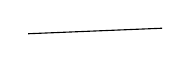
\begin{tikzpicture}
\draw (0,0) -- (1.7,0.07);
\end{tikzpicture}}

J'ai envie de présenter sous une forme légèrement différente la notion de L-groupe\inserted{ $\Pi$,} en termes de la donnée d'un $\mathbb Z$-module $T$ libre de rg $1$ (le $\mathbb Z$-module d'orientations) et d'un\deleted{\unsure{e}} \deleted{famille} \inserted{ensemble fini} $(k_i^{\unsure{\natural|\sharp}})_{i\in I}$ de \uline{germes} \uline{d'hom.} extérieurs
\[
\begin{gathered}
k_i^{\unsure{\natural|\sharp}}:\quad \deleted{\unsure{\mathbb Z}}\inserted{T}\longrightarrow\Pi
\qquad (i\in I)\\
(\text{\uline{germe} d'hom. ext.})
\end{gathered}
\tag{5}
\]
,

où la notion de ``germe'' est relative à celle des sous-groupes d'indice fini de $T$. \deleted{L'axiome à mettre est} \inserted{\unsure{Pour} une telle donnée,}

\scanpage{189}
\mspage{742}

et tout sous-groupe \deleted{\unsure{à}} $\Pi_0$ de $\Pi$ d'indice fini, on trouve \inserted{pour $\forall i$} un ens de germes d'hom extérieurs
\[
T\longrightarrow\Pi_0
\]
induits par les hom. \deleted{\unsure{ext.}} effectifs $nT\longrightarrow\Pi$ de la classe $k_i^{\unsure{\natural|\sharp}}$ --- on trouve un nb fini de germes d'hom. ext. $T\longrightarrow\Pi_0$ pour $i$ fixé, donc aussi pour $i$ variable dans $I$. Ceci dit, l'unique axiome d'une L-structure, c'est qu'on puisse trouver un sous-groupe $\Pi_0$ d'indice fini, tel que la ``structure induite'' provienne d'une structure à lacets de $\Pi_0$.

On peut généraliser la notion de L-structure, en s'inspirant de la définition précédente (p. ex), et en y laissant tomber l'exigence que $\Pi_0$ soit d'indice fini --- mais en

\scanpage{190}

prenant soin par contre que $\Pi_0$ soit \uline{distingué}. On exige que \deleted{les} pour $\forall i\in I$, les germes d'hom $k_i:\deleted{\unsure{n}}T\longrightarrow\Pi$ de la classe $k_i^{\unsure{\natural|\sharp}}$ se factorisent par $\Pi_0$ --- ce qui donne un ens. de \inserted{germes d'}hom extérieurs de $T$ dans $\Pi_0$ ---
\margin{NB il n'est pas clair a priori que cet ens. de germes d'hom. ext. soit fini}
et on exige que cette \deleted{ens. de} \inserted{structure-là} sur $\Pi_0$ provienne \inserted{(pour $\Pi_0$ convenable)} d'une structure à lacets sur $\Pi_0$, \unsure{$\xi$|\&} évidemment uniquement déterminée, une fois $\Pi_0$ choisi. Quant à $\Pi_0$, il est défini à commensurabilité près --- i.e. si $\Pi_0,\Pi'_0$ conviennent, alors $\Pi_0\inserted{\cap}\Pi'_0$ est d'indice fini dans $\Pi_0$ et $\Pi'_0$, et convient également.

\deleted{M'inspirant de la terminologie ``métabélienne'',} j'ai envie (à défaut d'une meilleure suggestion) d'appeler les groupes $\Pi$ munis d'une telle
